\chapter{\label{par_est}Parameter estimation using SOAP}
%%%%%%%%%%%%
%%%%%%%%%%%%
%%%%%%%%%%%%
%%%%%

Throughout Sec.~\ref{soap} and \ref{machine} we developed techniques which could identify whether a potential signal is present within a small frequency band ($0.1 Hz$) and return the most likely frequency track if the signal in that band.
This is useful information for all-sky searches as it can limit the parameter space for deeper searches such as those described in Sec.~\ref{searchcw:search:targeted}. 
However, this only limits the parameters space to a smaller frequency band, and potentially the frequency and derivative if we used the Viterbi track information.
This still leaves a large parameter space which a more sensitive method would have to search through.
In particular the sky position of the source has to be sampled finely as \gls{LIGO} can accurately localise a \gls{CW} source.
This is because the source is observed at multiple positions as the earth orbits sun, giving an effective aperture of the earth's orbital radius.
The SOAP search would therefore benefit if it could provide more information on the astrophysical source.

In this chapter I will outline a Bayesian method which uses the output Viterbi tracks of the SOAP search in Sec.~\ref{soap} to return some astrophysical parameters of a source.
Sec.~\ref{par_est:freq} will outline the model of the frequency evolution of a \gls{CW} from a source with a slowly varying frequency,
Sec.~\ref{par_est:bayes} will outline the Bayesian model for this analysis and Sec.~\ref{par_est:results} will show the results from testing on simulated signals.

%%%%
%%%%
\section{\label{par_est:freq}Pulsar frequency evolution}
%%%%
%%%%

The SOAP search returns a Viterbi track, where if this track follows the frequency of a pulsar signal, frequency evolution contains information of the sky position ($\alpha, \delta$) and the frequency of the source $f$ and its derivative $\dot{f}$ where we ignore higher order frequency derivatives.
From the Viterbi track, we should then be able to extract this information as we have a model for the phase evolution (and therefore frequency evolution) of the source described in Eq.~\ref{searchcw:model:phase} in Sec.~\ref{searchcw:model}.
To relate this phase evolution to the sky position parameters, we can look closer at Eq.~\ref{searchcw:model:ssbtime}, where we describe the shift in arrival time due to the earths motion. 

The second term in Eq.~\ref{searchcw:model:ssbtime} describes the Doppler shift due to the earth's orbit and rotation.
Where the $\bm{r}$ is the position of the detector and $\bm{n}$ is a unit vector in the direction of the source. 
As in \citep{schutz1998DataAnalysis}, we use the coordinate frame in the \gls{SSB} where the $z$ axis is perpendicular to the ecliptic and the $x$ axis is parallel to the celestial sphere.
In this frame the unit vector pointing towards the star can be written as 
\begin{equation}
    \label{par_est:freq:unit}
    \bm{n} = 
    \left(
    \begin{matrix}
        1 & 0 & 0  \\
        0 & \cos \epsilon & \sin \epsilon \\
        0 & -\sin \epsilon & \cos \epsilon \\
    \end{matrix} \right)
    \left(
    \begin{matrix}
        \cos(\alpha)\cos(\delta)  \\
        \sin(\alpha)\cos(\delta) \\
        \sin(\delta) \\
    \end{matrix} \right),
\end{equation}
where $\alpha$ and $\delta$ are the right ascension and declination (sky position) of the source and $\epsilon$ is the angle between the ecliptic and the earth's equator.
The first matrix in Eq.~\ref{par_est:freq:unit} describes a rotation from the \joe{earths} frame where $\alpha$ and $\delta$ are measured to the \gls{SSB} frame. 
The second matrix transforms the sky position parameters to their component $x,y,z$ coordinates.

The position vector of the earth at a time $t$, $\bm{r}$ in Eq.~\ref{searchcw:model:ssbtime}, can split into the addition of two components, the position due to the orbit of the earth and position due to the rotation of the earth.
The position of the earth in its orbit is described in cartesian coordinates as
\begin{equation}
    \bm{r}_{orb} = R_{\mathrm{O}}
    \left(
    \begin{matrix}
        \cos{\left( \Omega_{\mathrm{O}} t + \phi_{\omega){O}}  \right)}  \\
        \sin{\left( \Omega_{\mathrm{O}} t + \phi_{\omega){O}}  \right)} \\
        0 \\
    \end{matrix} \right),
\end{equation}
where $R_{\mathrm{O}}$ is the radius of the earth's orbit (1 AU), $\Omega_{\mathrm{O}}$ is the angular frequency of the earth's orbit $2\pi/T_{\mathrm{O}}$, where $T_{\mathrm{O}}$ is one year and $\phi_{\omega){O}}$ is some phase which defines the position of the earth in its orbital motion.
The position due to the rotation of the earth can then be described by 
\begin{equation}
    \bm{r}_{rot} = R_{\mathrm{R}}
    \left(
    \begin{matrix}
        1 & 0 & 0  \\
        0 & \cos \epsilon & \sin \epsilon \\
        0 & -\sin \epsilon & \cos \epsilon \\
    \end{matrix} \right)
    \left(
    \begin{matrix}
        \cos{(\lambda)}\cos{\left( \Omega_{\mathrm{R}} t + \phi_{\omega){R}}  \right)}  \\
        \cos{(\lambda)}\sin{\left( \Omega_{\mathrm{R}} t + \phi_{\omega){R}}  \right)} \\
        \sin{(\lambda)} \\
    \end{matrix} \right),
\end{equation}
where $R_{\mathrm{R}}$ is the radius of the earth, $\Omega_{\mathrm{R}}$ is the angular frequency of the earth's rotation $2\pi/T_{\mathrm{R}}$, where $T_{\mathrm{R}}$ is one day, $\phi_{\omega){O}}$ is some phase which defines the position of the earth in its rotational motion and $\lambda$ is the latitude of the detectors site.
These two components can then be added to find the location of the detector in the \gls{SSB} frame
\begin{equation}
    \bm{r} = \bm{r}_{orb} + \bm{r}_{rot}.
\end{equation}

We can now describe the phase evolution of the signal at the detectors site from just the sky position ($\alpha, \delta$) and frequency and its derivative $f,\dot{f}$. 
The frequency of a pulsars signal at any point on the frequency track is then defined by the derivative of the phase with respect to time
\begin{equation}
    f = \frac{d\Phi}{dt}, 
\end{equation}
where $\Phi$ is defined in Eq.~\ref{searchcw:model:phase}.
\joe{maybe add the actual frequency evolution equation}

%
%
\section{\label{par_est:bayes}Bayesian Model}
%
%

As described in Sec.~\ref{par_est:freq} we have a model of a pulsars frequency evolution and we have our Viterbi track which is our observation of a frequency track.
We would now like to estimate the parameters $\bm{\theta} = \left\{\alpha, \delta, f, \dot{f} \right\}$ of a pulsar given that we have observed the frequency track $\bm{V}$.
To do this we use a Bayesian model, where the idea was introduced in Sec.~\ref{intro:prob:bayes}, where we rewrite Bayes formula in terms of this problem
\begin{equation}
    \label{par_est:bayes:eqn}
    p(\bm{\theta} \mid \bm{V}, I) = \frac{p(\bm{\theta}) p(\bm{V} \mid \bm{\theta}, I)}{p(\bm{V} \mid I)}
\end{equation}
where $p(\bm{\theta} \mid \bm{V}, I)$ is the posterior which we are interested in, $p(\bm{\theta})$ is the prior, $p(\bm{V} \mid \bm{\theta}, I)$ is the likelihood and $\bm{V} \mid I)$ is the evidence.
The following sections will describe how we set up the prior and likelihood for this problem.

%
%
\subsection{\label{par_est:bayes:likelihood}Likelihood}
%
%

The likelihood describes how the noise of the data is distributed, i.e. if we subtracted the model frequency track from our observed frequency track, what is the distribution of these values.
If the simulated pulsar signal has an infinitely large \gls{SNR} then the Viterbi track would follow the pulsars frequency track exactly, which would leave a noise distribution of 0 with no variance. 
If conversely, the \gls{SNR} was zero then the Viterbi track would wander randomly through the frequency band and the noise would have a large variance in frequency.
The noise distribution of a Viterbi track, is then dependent on the \gls{SNR} if the signal within the band.
As the distribution of the noise is unknown analytically, we calculate it empirically using many simulated signals.

In Sec.~\ref{soap:results} we generated $\mathcal{O}(10^{4})$ simulated signal which, amongst other quantities, saved the Viterbi track, the simulated pulsar frequency track and the signals \gls{SNR}, $\rho$.
These simulations had \glspl{SNR} between 50 and 150, \joe{might update to 20-200}.
We can estimate the noise distribution by taking the \gls{KDE} of the differences between the Viterbi and pulsar frequency tracks for all simulations in a given \gls{SNR} range.
We split the likelihood into 90 discrete bins, each of which are \gls{SNR} 2 wide, where this ranges from \gls{SNR} 20 to 200.
Figure \ref{par_est:bayes:likelihood:kde142} shows an example of the \glspl{KDE} of a subset of the likelihood bins. 
The sharp peaks in the center of each sub plot in Fig.~\ref{par_est:bayes:likelihood:kde142} represents simulations where the Viterbi track is close to the simulated pulsar track, and the broader distributions represent areas of the Viterbi track has not identified the pulsar track but is wandering randomly.
The sub plots in Fig.~\ref{par_est:bayes:likelihood:kde142} show that as the \gls{SNR} increases the distribution is more closely centred around 0, i.e. the Viterbi and pulsar tracks are similar, which is expected.
%
\begin{figure}[ht]

    \centering
    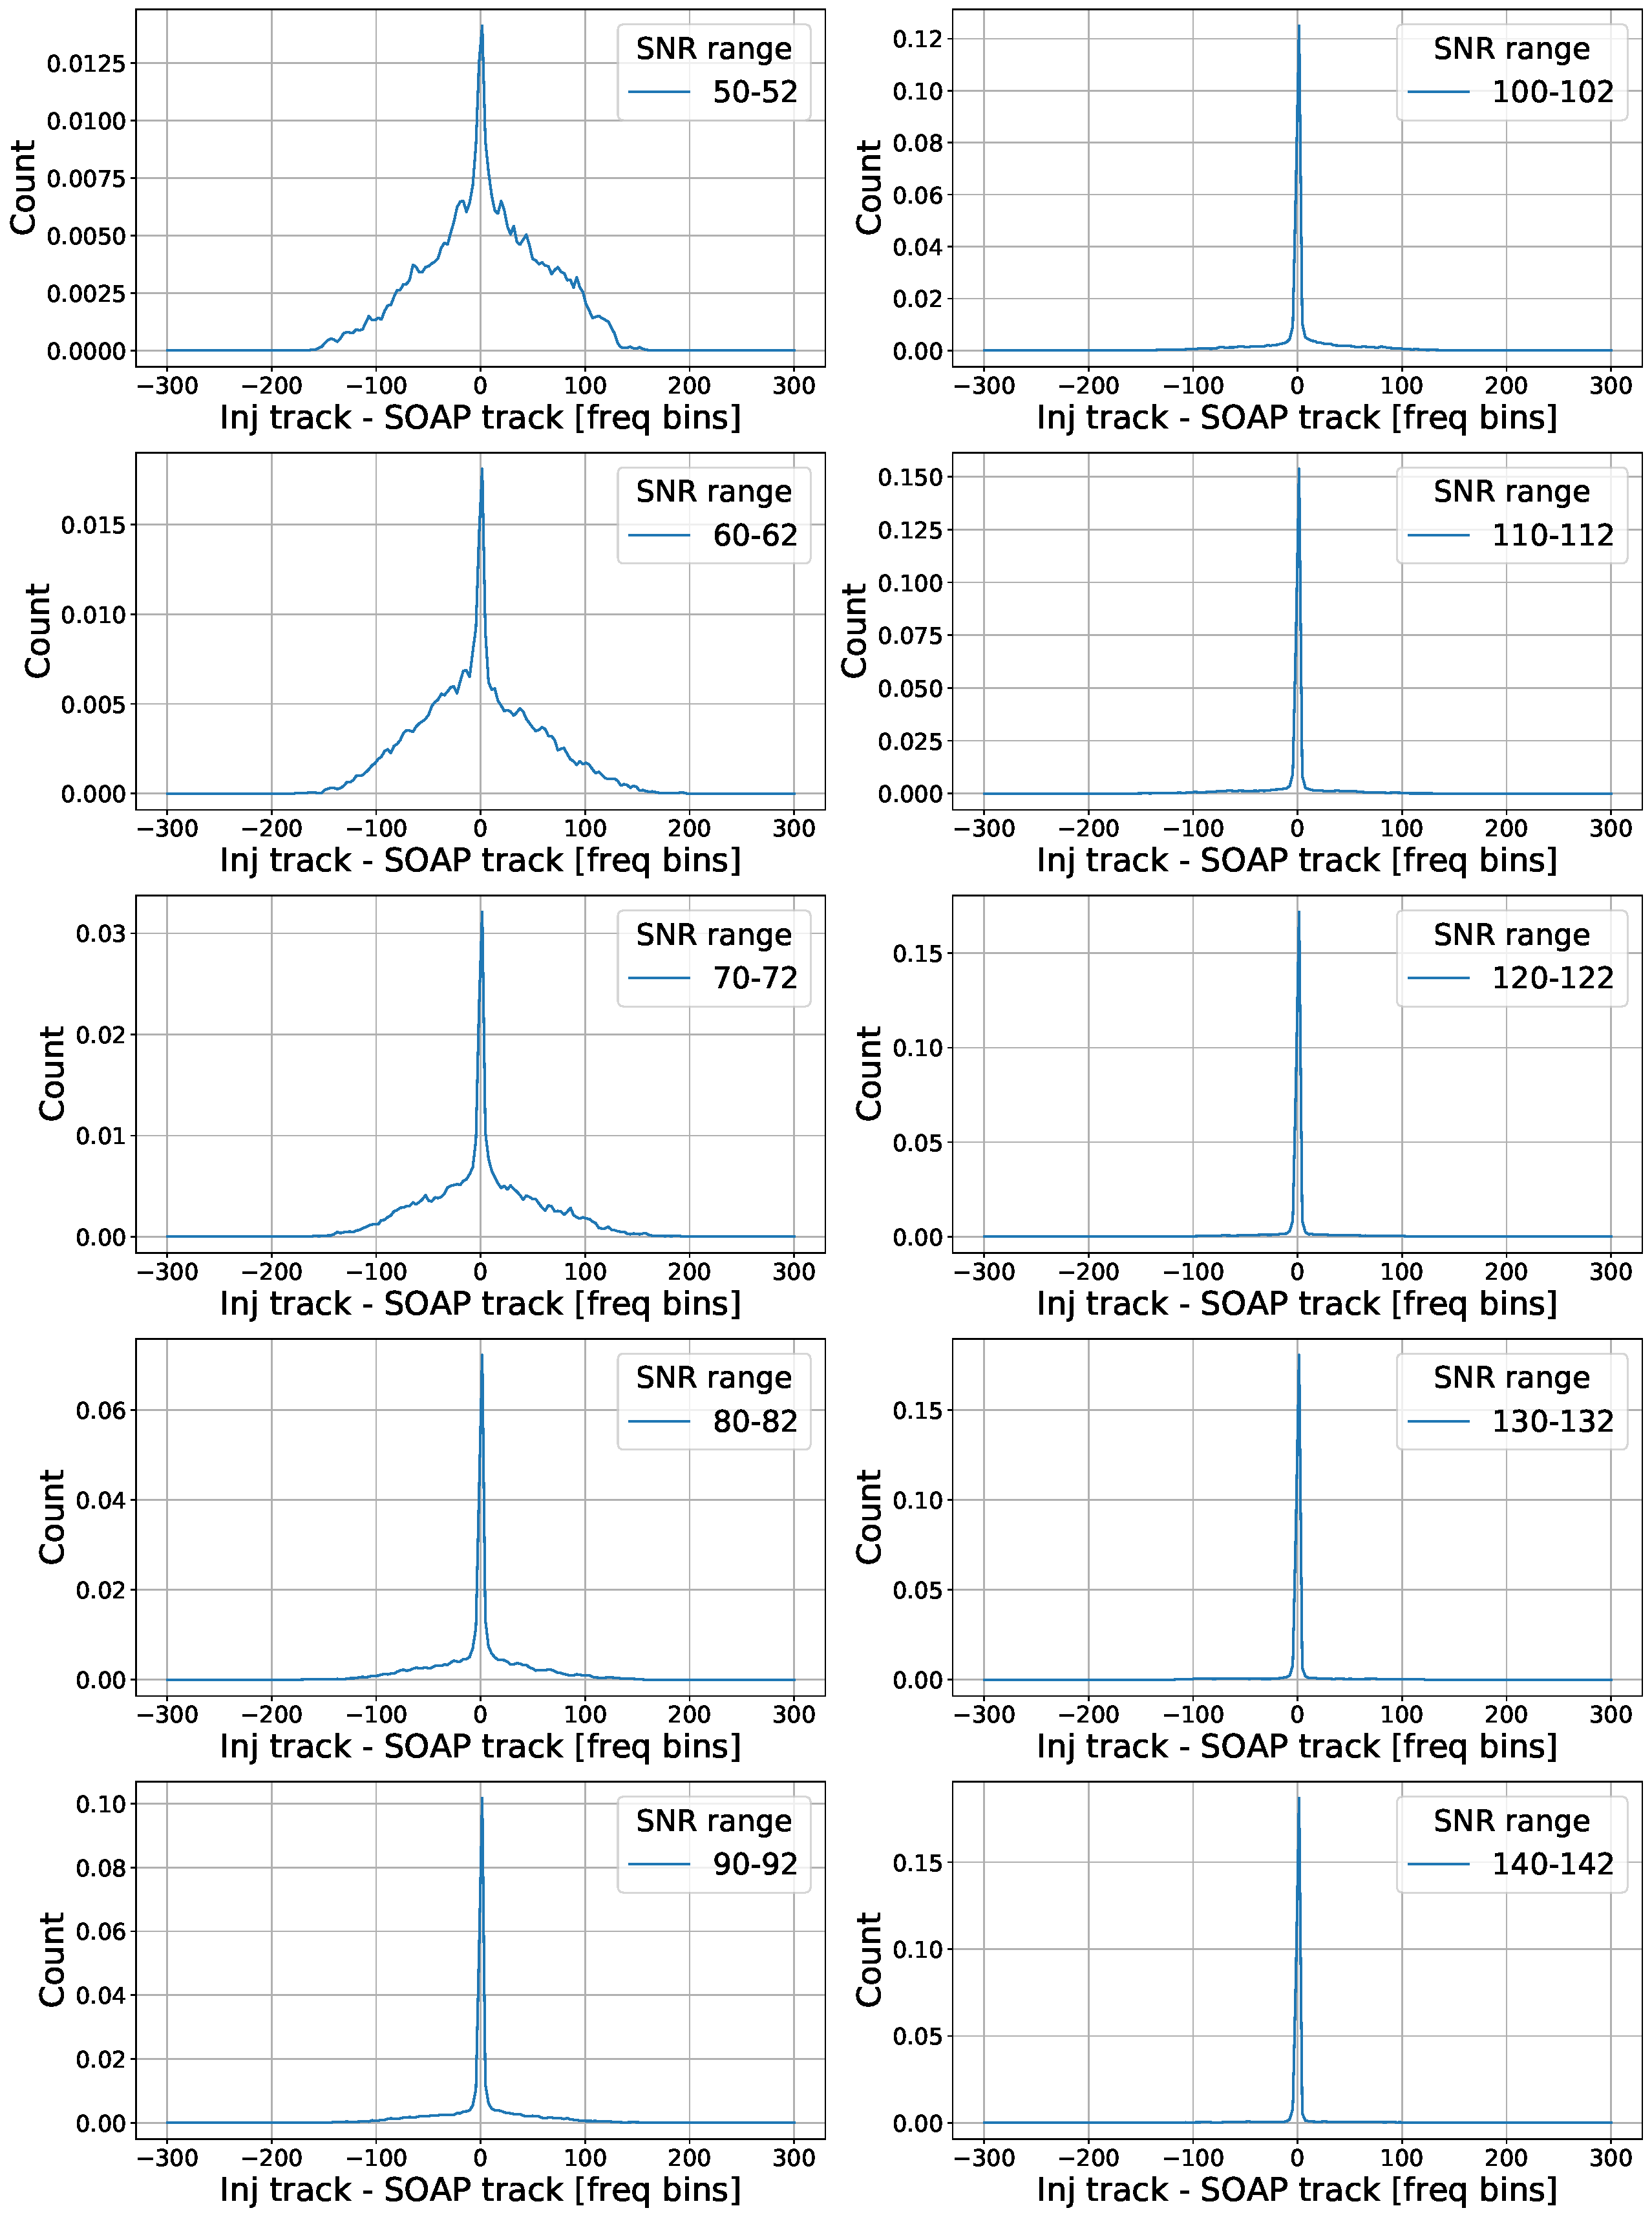
\includegraphics[width=\linewidth]{C5_parameter/KDE_range_50_100.pdf}
    \caption[KDE of likelihood in different \gls{SNR} ranges]{This figure shows the \gls{KDE} estimates of the probability density of the differences between the simulated (injected) pulsar frequency track and the recovered Viterbi track for a number of \gls{SNR} ranges. The difference in the tracks is measured in discrete frequency bins. Each \gls{KDE} is generated from $\sim 300$ simulations which each have $\sim 400$ elements in their frequency tracks. This shows a subset of the binned likelihoods between the range of \gls{SNR} 50 and 150.}
    \label{par_est:bayes:likelihood:kde142}
    
    \end{figure}
%

This does introduce one more parameter to search over in out Bayesian model, which is the \gls{SNR} ($\rho$) of the signal.
These \glspl{KDE} are the used as the likelihood function $p(\bm{V} \mid \bm{\theta}, I)$ in the Bayesian model in Eq.~\ref{par_est:bayes:eqn}, where we not have five parameters $\bm{\theta} = \left\{\alpha, \delta, f, \dot{f} , \rho \right\}$.


%
\subsection{Prior}
%
We set up a simple prior which does not assume much about the parameters, other than limits on their range. 
We use a flat prior for $\alpha$ between $[0,2\pi]$, a flat prior in $\sin{\delta}$ between [-1,1], a flat prior in $f$ in the range of the 0.1 Hz wide sub-band which SOAP searched through and a flat prior in the frequency derivative in the range $[-1\cdot 10^{9},1\cdot 10^{9}]$.
The prior for $\rho$ is also flat in the range $[50,200]$.

%%%%
%%%%
\section{Results}
%%%%
%%%%

For the tests of this method, we generate a pulsar signal in a spectrogram and run the SOAP search as in Sec.~\ref{soap:results} and \ref{machine:results}.
In each of these we record the Viterbi track and the pulsar signal parameters $\alpha, \delta, f, \dot{f} , \rho$ associated with the pulsars frequency track.
This contains the information needed to run the bayesian analysis described in Sec.~\ref{par_est:bayes}.
We generated signals with the parameters as described in Tab.~\ref{}, which had an \gls{SNR} range between 20 and 200\joe{check}, and frequency ranges between 40 and 500 Hz \joe{check}.
However, as the \gls{SNR} is the simulations decreases, the probability of SOAP identifying the signal decreases. 
As this analysis is intended to be the first stage of a follow up of those results, we use the detection statistics mentioned in Sec.~\ref{soap:results} to identify `detected' signals.
In these sections, we set a 1\% false alarm rate to generate efficiency curves, therefore, for this analysis we use the top 1\% of Viterbi statistics from this search band for a follow up analysis.

As an example of what is returned by the Bayesian analysis described in Sec.\ref{par_est:bayes}, Fig.~\ref{par_est:results:example_posterior} shows the returned marginal posterior distributions for each of the parameters in the search.

\begin{figure}[pt]

    \centering
    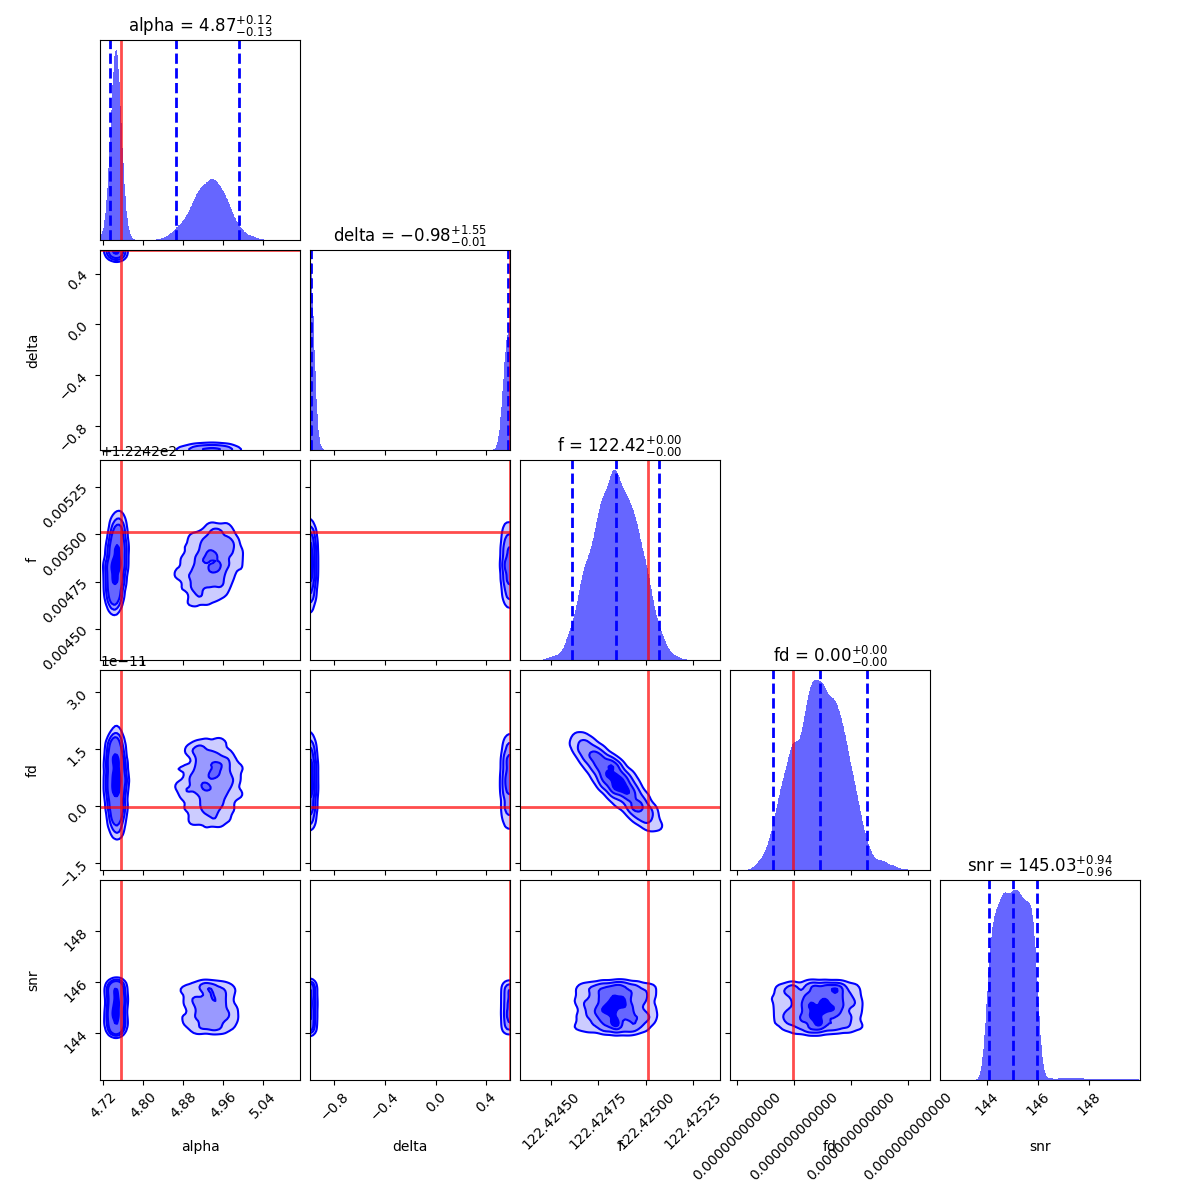
\includegraphics[width=\linewidth]{C5_parameter/cornerplot.png}
    \caption[KDE of likelihood in different \gls{SNR} ranges]{This figure shows an example of the posterior distribution of a signal with \gls{SNR} \joe{SNR}. Each panel shows the marginal distributions for each parameter, where the parameters used for the simulation are marked in red.}
    \label{par_est:results:example_posterier}
    
\end{figure}
%

As mentioned above \joe{mention above}, one of the largest issues with all-sky searches is the number of templates needed to sufficiently cover the parameter space in sky position. 
Therefore, the marginal posterior for the sky position can be plotted for a \joe{words} of the position as shown in Fig.~\ref{}.
The Viterbi tracks and pulsar frequency tracks used in this analysis are sampled once a day, therefore, we should only see the doppler modulation from the orbit of the earth around the sun.
In the ecliptic frame, i.e. where the $z$ axis is perpendicular to the orbital plane of the earth, for any ecliptic longitude, there are two sky positions at opposite ecliptic latitudes which will return the same frequency track. 
This then means that we would expect the posterior distribution to have two modes on the sky at these two locations, where this can be seen in Fig.~\ref{} and \ref{}.
The sky position parameters of the pulsar are in the equatorial coordinate system, i.e. the earth as the reference frame, therefore have been transformed into the Ecliptic frame to make the sky position posteriors easier to read and understand.
%
\begin{figure}[ht]
    \centering
    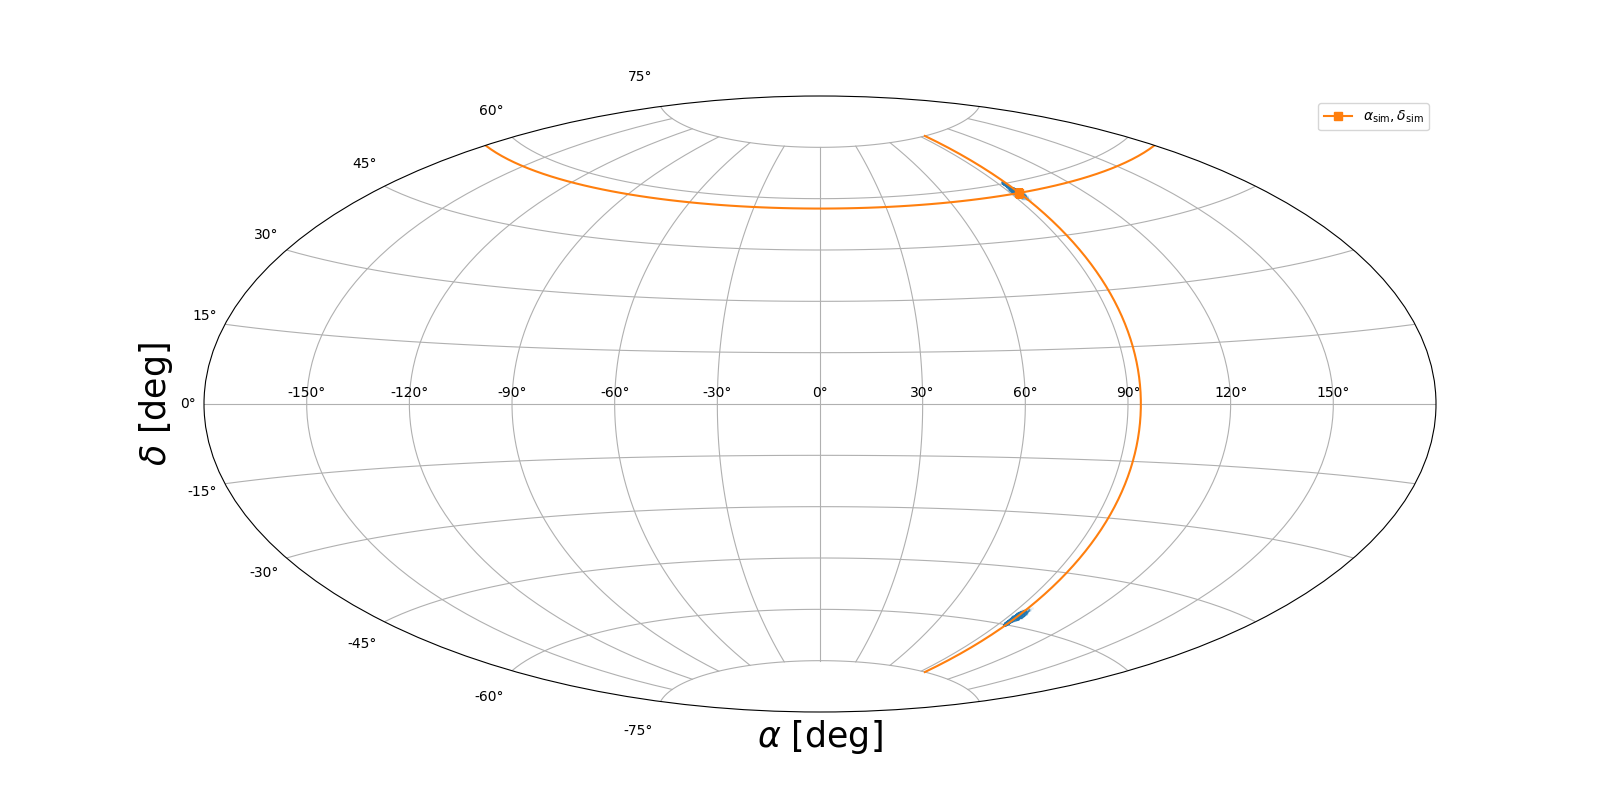
\includegraphics[width=\linewidth]{C5_parameter/skypos_ecliptic.png}
    \caption[Example of posterior of sky position]{This figure shows an example of the marginal posterior distribution of the sky position of a signal with \gls{SNR} \joe{SNR}. The coordinates are in the ecliptic frame.}
    \label{par_est:results:example_posterier}
    
\end{figure}
%

\section{searching over many signals section \joe{need a name}}

To test this analysis, the Bayesian method in Sec.~\ref{par_est:bayes} is run on the simulation which had Viterbi statistics within the top 1\% of those in the search band between 40 and 500 Hz.
For each of these simulations, the analysis returns a posterior distribution of the parameters.

One method to asses the ability of this to identify the correct parameters is the p-p plot.
\joe{need better description of p-p plot}

This is calculated using the marginal distributions for each of the parameters.
In Fig.~\ref{} we show the p-p plot which was generated from \joe{top 1\%} 200 simulated signals.
If the plots lie along the diagonal line, this means that the posterior distributions agree with the simulated parameters, whereas line which are far away from this indicate that the parameters are not consistent with the injections.

Figure \ref{ppplot} shows that the simulated signals are not completely consistent with the injected parameters for the \joe{which parameters}


Another method to asses the power of this analysis in terms of locating the sky positions of the source is the measure the area on the sky which this can localise to.
To do this 




\joe{say what reduction in sky area is useful for passing on to future searches}